

\documentclass[12pt]{book}
%\usepackage[paperwidth=6in,paperheight=9in,margin=1.2in]{geometry}
\usepackage[a4paper]{geometry}

\usepackage{mystyle}
\usepackage{hyperref}
 
\title{TrainABA Supervision Curriculum Series\\ Volume 1: BCBA Reference Manual \\Second Edition}
\author{B. Theisen}
\date{April 21, 2019}
\makeindex[intoc]
 \renewcommand*{\marginfont}{\color{NavyBlue}\bfseries\sffamily}
\begin{document}
%include{path/to/title.tex}
     \maketitle
     \tableofcontents
     \listoffigures
     \listoftables
%% Uncomment sections to be included here. 
%% Note that sections cannot be nested. List everything here. Treat this text file as the sole index for calling which sections  to include in the book you are compiling.
 

\documentclass[float=false, crop=false]{standalone}
\usepackage[subpreambles=true]{standalone}
\usepackage{import}
\begin{document}
\chapter{Introduction}
To kick it off, here is a view of space. 
\index{space}
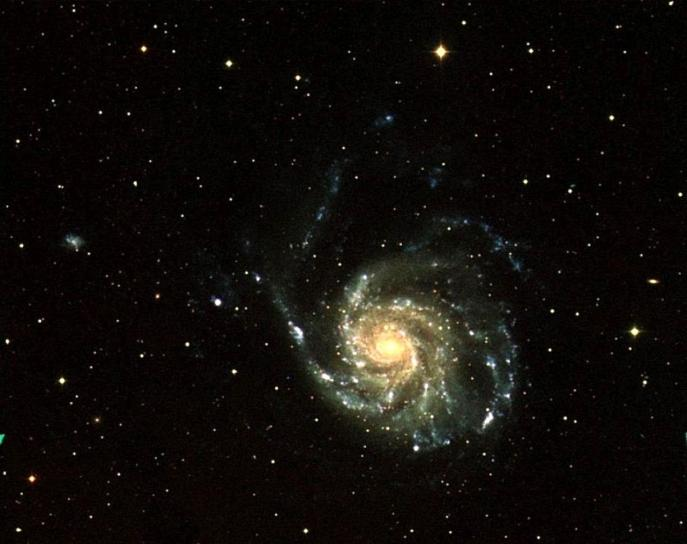
\includegraphics[scale=0.2]{space}
However, the image is only the beginning. Wait until the next chapter to see the image as a figure!

A TikZ figure will be rendered below this line...
 
 
\begin{figure}[ht]
 
\subimport{../}{diagram.tex}
 
\label{fig:tikzexample}
\caption{A nice simple diagram}
\end{figure}
 
...
\end{document}



 

\documentclass[float=false, crop=false]{standalone}
\usepackage[subpreambles=true]{standalone}
\usepackage{import}
\begin{document}
\chapter{Administration}
This is a whole chapter about administration for supervisors. None of it is dependent on implementing procedures of certification or licensing entitities. For example, \underline{\texttt{\colorbox{Dandelion}{Fourier series}}}
\marginnote{Fourier Series}
\index{Fourier series}
gets indexed for no apparent reason.

Say, do you remember that image of space from last chapter? Here is the image, presented as a figure. Look how pretty a figure can be!
\begin{figure}[h]
    \centering
    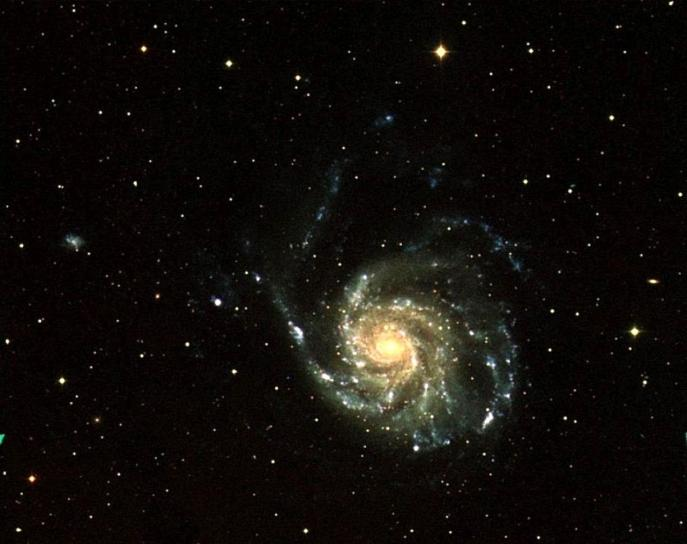
\includegraphics[width=0.25\textwidth]{space}
    \caption{A nice space.}
    \label{fig:space1}
\end{figure}
 
As you can see in the figure \ref{fig:space1}, the 
function grows near 0. Also, in the page \pageref{fig:space1} 
is the same example.
 
All of this continues to another page, which includes a bulleted list.
\begin{itemize}
\item fun
\item sun 
\item rock
\item roll
\item magic
\item fun
\item space
\item more
\item okay
\end{itemize}


The most important consideration is the use of power when microwaving burritos. Whether at a concert or anywhere that sells gasoline, burritos and microwaves are your friends. These are the friends you want to keep. Parents encourage their kids to have these lasting relationships. 

A \textcolor{orange}{TikZ}
\marginnote{TiKZ} 
\index{TikZ}
 figure will be rendered below this line. It has to get to the next page first. Be sure to hold your excitement for the moment. It really will be ready to show momentarily. Any old moment. Could be this one. Maybe now? 
 \begin{figure}[ht]
 \subimport{../}{diagram.tex}
 \label{fig:tikzexample}
\caption{A nice simple diagram}
\end{figure}
 ...
\end{document}



      \printindex
\end{document}



